Nei capitoli precedenti abbiamo visto come è possibile connettere reti locali tramite una rete IP pubblica, fornendo accesso a internet.
Presentiamo prima però le due strategie principali per permettere la comunicazioni tra reti:
\begin{itemize}
	\item \textbf{Connettività generale}: l'accesso a internet è garantito da un ISP (usata per utenti residenziali).
	Strutturata in modo gerarchico, composta da diverse reti organizzare in autonomous system (AS). L'instradamento è garantito da IGP (Interior Gateway Protocol) all'interno di un AS e da EGP (Exterior Gateway Protocol) tra AS.
	\item \textbf{Connettività dedicata}: tipicamente usata per connettere sedi aziendali (uso business). Viene offerta da specifici ISP. In generale è una soluzione molto più costosa. Viene anche chiamata \textbf{WAN}.
	
\end{itemize}
\section{Wide area networks (WAN)}
Nelle reti a connettività dedicata è necessario fornire una garanzia di qualità del servizio (QoS) per assicurare che le prestazioni siano adeguate alle esigenze dell'utente.
\begin{figure}[H]
	\centering
	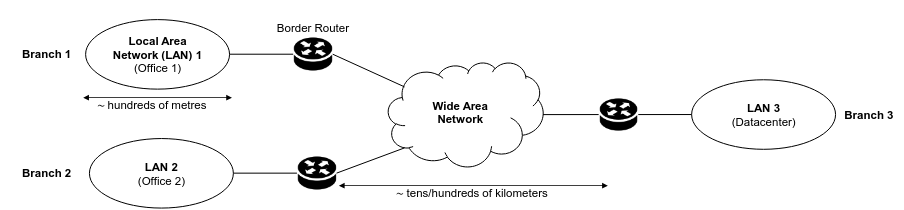
\includegraphics[width=\textwidth]{pictures/3/wan.png}
	\caption{Esempio di WAN}
\end{figure}
\subsection{Soluzioni}
È possibile adottare diverse tecnologie per implementare una WAN, tra cui:
\subsubsection{WAN dedicata fisica}
L'azienda possiede l'infrastruttura di rete e la gestisce direttamente.
	\begin{itemize}
		\item Controllo completo sulla rete, banda molto elevata, ma la gestione della sicurezza è a carico dell'azienda.
		\item Costi elevati, possibilmente ridotti dall'utilizzo della fibra oscura.
	\end{itemize}
\begin{figure}[H]
	\centering
	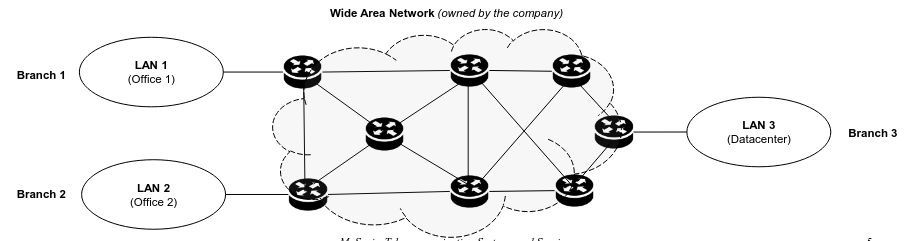
\includegraphics[width=0.9\textwidth]{pictures/3/dedicated_wan.png}
	\caption{Esempio di WAN dedicata fisica}
\end{figure}
\subsubsection{Linee in affitto}
L'azienda stipula un contratto con un operatore di rete che crea una connessione dedicata tra le sedi dell'azienda.
\begin{itemize}
	\item Questi circuiti privati possono essere realizzati come lunghezze d'onda dedicate su fibra ottica (wavelength-division multiplexing, WDM) o come circuiti TDM (time-division multiplexing).
	\item Il controllo sulla rete è limitato, dato che il controllo della sicurezza è a carico dell'operatore di rete.
	\item Rimane una soluzione costosa.
\end{itemize}
\begin{figure}[H]
	\centering
	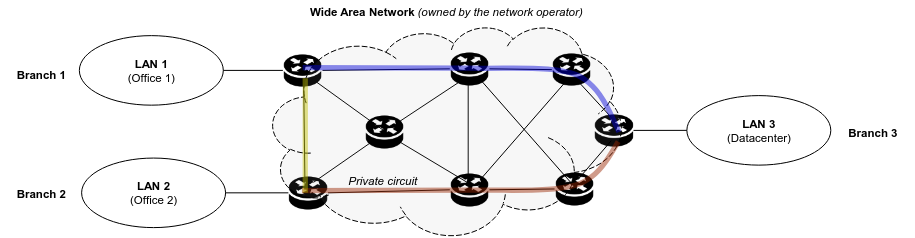
\includegraphics[width=0.9\textwidth]{pictures/3/leased_wan.png}
	\caption{Esempio di WAN con linee in affitto}
\end{figure}
\subsubsection{Multiprotocol level switching (MPLS)}
L'azienda stipula un contratto con un operatore di rete che fornisce una connessione mesh con certe garanzie di QoS.
È una soluzione più economica rispetto alle linee in affitto, ma con un controllo limitato sulla rete.
\begin{figure}[H]
	\centering
	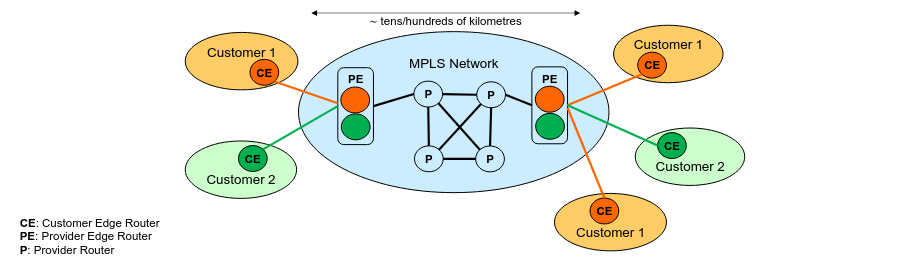
\includegraphics[width=0.9\textwidth]{pictures/3/mpls_wan.png}
	\caption{Esempio di WAN con MPLS}
\end{figure}
In particolare ci concentriamo su questa soluzione.
\subsection{Multiprotocol level switching}
Iniziamo ricordando come funzione il routing IP.
Il routing è un processo che definisce come i pacchetti vengono instradati da una sorgente a una destinazione attraverso una rete.
Si basa sul \textbf{destination based forwarding}. Gli elementi fondamentali del routing sono:
\begin{itemize}
	\item \textbf{Routing table}
	\item \textbf{Routing algorithms}
\end{itemize}
L'architettura MPLS permette di gestire circuiti virtuali per flussi di dati. 
Questi flussi possono essere predeterminati dall'operatore di rete o stabiliti dopo una richiesta da parte dell'utente.
La creazione di questi flussi quando necessario avviene tramite un processo di set up e prenotazione di una risorsa.
\begin{figure}[H]
	\centering
	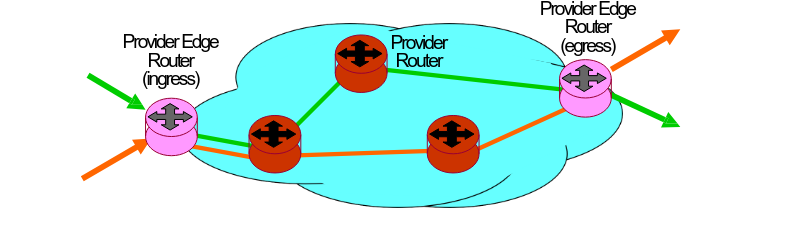
\includegraphics[width=0.9\textwidth]{pictures/3/archi_mpls.png}
	\caption{Architettura MPLS}
\end{figure}\noindent
I flussi di dati possono essere ottimizzati in maniera dinamica. Inoltre, è possibile instradare il traffico secondo criteri diversi da quelli basati sulla destinazione.
\subsection{Label swapping forwarding}
Spostiamo il paradigma del routing da destination based forwarding a label swapping forwarding.
Un pacchetto IP viene incapsulato in un header MPLS (32 bit), detto anche \textbf{shim header}, \textbf{MPLS label} o semplicemente \textbf{label}.
Viene aggiunto tra l'header di livello 2 (L2) e quello di livello 3 (L3).
È possibile incapsulare più label, creando una pila di label (label stack).
\begin{figure}[H]
	\centering
	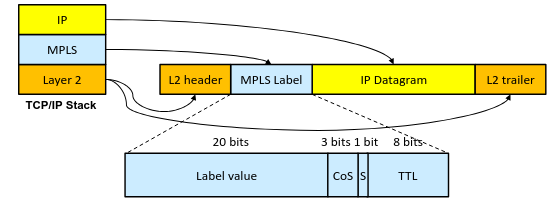
\includegraphics[width=0.9\textwidth]{pictures/3/label_swapping.png}
	\caption{Label swapping forwarding}
\end{figure}\noindent
un label è composto da 4 campi:
\begin{itemize}
	\item \textbf{Label value} (20 bit): identifica il flusso di dati a cui il pacchetto appartiene.
	\item \textbf{Traffic class} (3 bit): usato per la QoS, permette di classificare i pacchetti in base alla priorità.
	\item \textbf{Bottom of stack} (1 bit): indica se il label è l'ultimo della pila (il più interno).
	\item \textbf{Time to live} (8 bit): usato per evitare loop di routing, decrementato ad ogni hop.
\end{itemize}
Le label vengono quindi usate dai router per fare forwarding dei pacchetti tramite label swapping.
Quando un pacchetto arriva sostituisce la in-label con una out-label, e inoltra alla interfaccia associata alla out-label.
L'associazione label-interfaccia è definita da una tabella di forwarding.
Così facendo, si crea un circuito virtuale tra la sorgetente e la destionazione (provider edge routers).
Le label hanno un significato locale, quindi possono essere riusate in diverse parti della rete.
In realtà, la nomenclatura più specifica per queste componenti è:
\begin{itemize}
	\item provider edge router (PE) $\rightarrow$ \textbf{Label Edge Router (LER)}
	\item provider router (P) $\rightarrow$ \textbf{Label Switch Router (LSR)}
	\item Virtual circuit $\rightarrow$ \textbf{Label Switched Path (LSP)}
\end{itemize}
\begin{figure}[H]
	\centering
	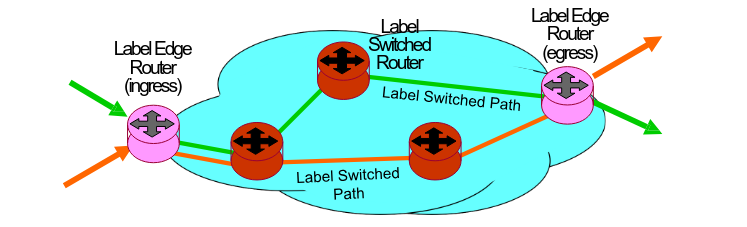
\includegraphics[width=0.9\textwidth]{pictures/3/archi_mpls_specific.png}
	\caption{Architettura MPLS con nomenclatura specifica}
\end{figure}
Le label vengono rimpiazzate dal LSR durante la fase di label swapping. Le label sono associate tra loro e con le interfacce durante la fase di set up del percorso.
\begin{figure}[H]
	\centering
	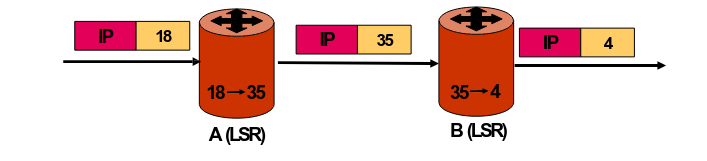
\includegraphics[width=0.9\textwidth]{pictures/3/lsr-lsr.png}
	\caption{Label swapping tra LSR}
\end{figure}\noindent
Al label edge router (LER) \underline{ingress} c'è una corrispondenza tra indirizzo di destinazione e prima label sul percorso.
\begin{figure}[H]
	\centering
	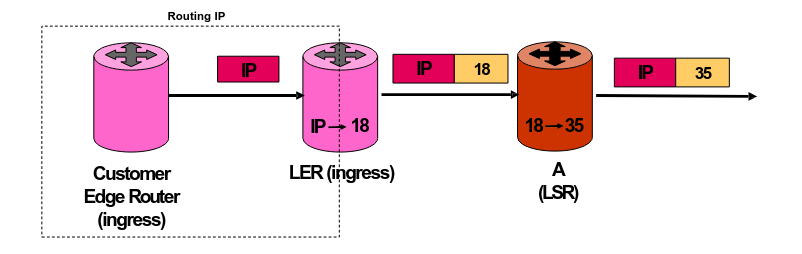
\includegraphics[width=0.9\textwidth]{pictures/3/ler_ingress.png}
	\caption{Label edge router (LER) ingress}
\end{figure}\noindent
Al label edge router (LER) \underline{egress} il routing avviene tramite IP.
\begin{figure}[H]
	\centering
	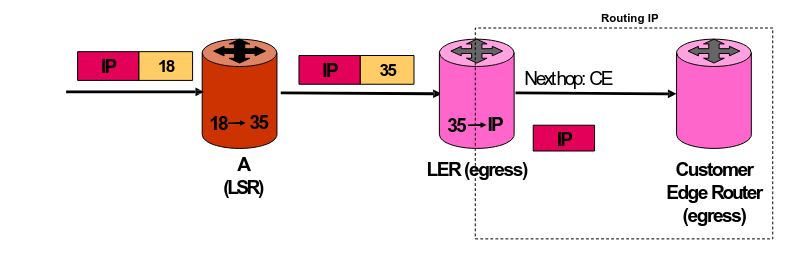
\includegraphics[width=0.9\textwidth]{pictures/3/ler_egress.png}
	\caption{Label edge router (LER) egress}
\end{figure}
\subsubsection{Esempio}
Supponiamo di avere due LSP che seguono un percorso comune A-C.
\begin{figure}[H]
	\centering
	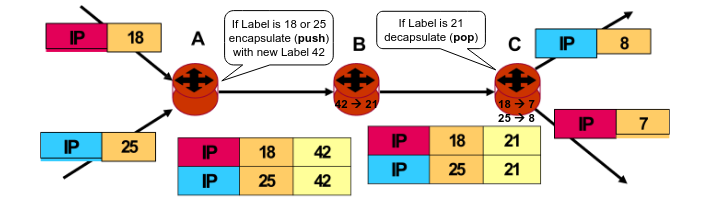
\includegraphics[width=0.9\textwidth]{pictures/3/path_binding.png}
	\caption{Esempio di due LSP che seguono un percorso comune A-C}
\end{figure}
\begin{itemize}
	\item A incapsula i pacchetti associati ai due LSP che usano la stessa label (42).
	\item B instrada i pacchetti considerando le outer label (42) e la sostituisce con la label (21) associata al percorso B-C.
	\item C decapsula l'outer label (21) e instrada i pacchetti in base alla inner label.
\end{itemize}
Possiamo fare qualche considerazione su questo esempio:
\begin{itemize}
	\item Non ci sono limiti ai binding di flusso.
	\item Il forwarding del traffico da parte dei router è basato su operazioni di swapping, popping e pushing di label.
	\item Questo meccanismo offre ottima scalabilità dato che i router possono effettuare operazioni di swapping su poche label.
\end{itemize}
\subsection{LS vs. destination based forwarding}
Il destination based forwarding è basato sull'indirizzo di destinazione, le tabelle di routing contengono prefissi di indirizzi di destinazione, e fanno il match più lungo possibile.
Per definizione il traffico non viene distinto in base alla sorgente, QoS, o altri criteri.
Il label swapping forwarding è basato su label che vengono scambiate ad ogni nodo. 
È inerentemente orientato alla connessione, dato che i pacchetti vengono associati a flussi di dati.
Una volta configurato, le tabelle di forward assicurano che il traffico associato a un LSP (generalmente chiamato flusso) segue sempre il percorso associato al LSP.
Il matching delle label è esatto.
\subsection{Forwarding e traffico di controllo}
La possibilità di creare cammini di swap di label permette di fare traffic engineering, ovvero di instradare il traffico in modo da ottimizzare l'utilizzo della rete.
Possiamo in questo modo creare i cammini in modo automatizzato. Ovviamente i dati di traffico e di controllo vengono trattati in modo differente.
\begin{itemize}
	\item \textbf{Pacchetti di controllo}: usati per la creazione automatica di cammini di label switching, tipicamente gestiti in modo simile al routing IP.
	\item \textbf{Pacchetti di dati}: usati per il forwarding dei pacchetti, forwarding basato su label swapping. 
\end{itemize}
Ovviamente, è possibile anche creare cammini di label switching in modo manuale, ma è una soluzione poco scalabile.
\subsection{Traffic engineering database (TED)}
\begin{figure}[H]
	\centering
	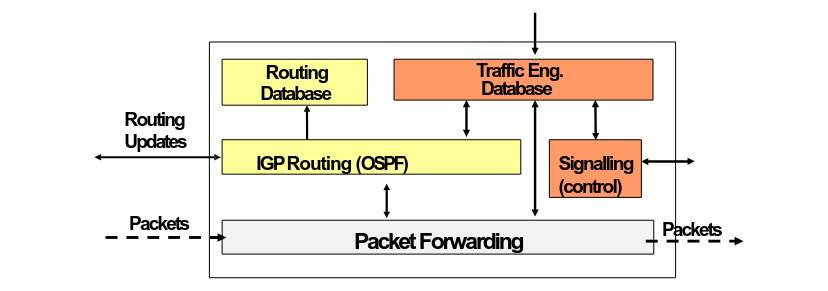
\includegraphics[width=0.9\textwidth]{pictures/3/TED.png}
	\caption{Traffic engineering database (TED)}
\end{figure}\noindent
Per effettuare network engineering viene introdotto un nuovo componente, il \textbf{traffic engineering database (TED)}.
Il TED contiene:
\begin{itemize}
	\item Informazioni topologiche della rete (ottenute tramite protocolli di routing).
	\item Informazioni sulle risorse della rete, come la capacità e lo stato dei link (ottenute tramite estensioni di protocolli di routing).
\end{itemize}
Grazie a queste informazioni è possibile effettuare LSP.
MPLS permette di effettuare routing basato su criteri, come ad esempio la QoS, che non sono basati sulla destinazione.
Di conseguenza, gli LSP possono essere creati in modo da soddisfare specifici requisiti. Il calcolo degli LSP può essere fatto offline (effettuando una ottimizzazione globale, a patto di conoscere a priori le richieste di traffico) o online (calcolando gli LSP in tempo reale).
È dunque necessario usare un meccanismo di signaling per:
\begin{itemize}
	\item Coordinare la distribuzione di label.
	\item Creare i percorsi desiderati.
	\item Prenotare, rilasciare e riallocare risorse.
	\item Evitare cicli.
\end{itemize}
Ci sono tre possibili meccanismi di signaling:
\begin{itemize}
	\item \textbf{Label Distribution Protocol (LDP)}: Hop-by-hop, distribuisce label per ogni prefisso di destinazione seguendo i protocolli IGP, non supporta il traffic engineering.
	\item \textbf{Constraint-Based Routing LDP (CR-LDP)}: Estensione di LDP per supportare il traffic engineering e il routing esplicito.
	\item \textbf{Resource Reservation Protocol-Traffic Engineering (RSVP-TE)}: Soluzione più complessa che supporta nativamente il traffic engineering e il routing esplicito.
\end{itemize}
\subsection{RSVP-TE}
La sorgente manda un messaggio PATH verso la destinazione (routing esplicito), impostando quindi il cammino su cui viene fatta la richiesta.
La destinazione accetta la richiesta e risponde con un messaggio RESV, che viene inoltrato lungo il cammino inverso.
A differenza di LDP, le label non vengono distribuite hop-by-hop, ma dal destination LER a tutti i router del cammino.
\begin{figure}[H]
	\centering
	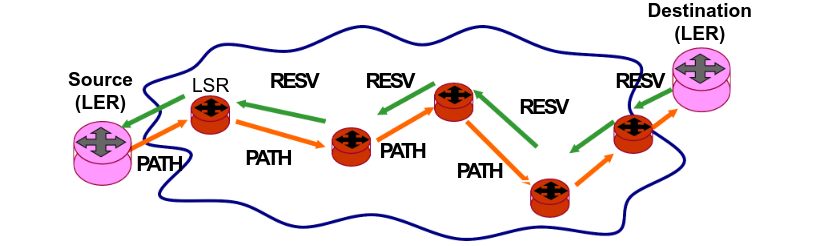
\includegraphics[width=0.9\textwidth]{pictures/3/rsvp.png}
	\caption{Esempio di signaling con RSVP-TE}
\end{figure}\noindent
Per poter fare traffic engineering è possible creare LSP su cammini con risorse libere, senza dover seguire i cammini più brevi.
Il consumo di banda su un cammino può essere stimato a priori o calcolato dinamicamente.
\begin{figure}[H]
	\centering
	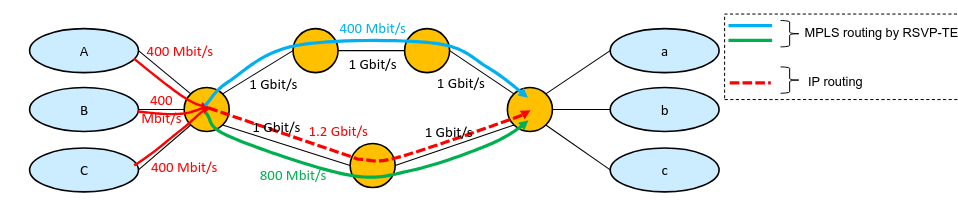
\includegraphics[width=0.9\textwidth]{pictures/3/rsvp_engineering.png}
	\caption{Esempio di traffic engineering con RSVP-TE	}
\end{figure}
Gli LSP vengono quindi creati seguendo criteri di risorse necessarie, affidabilità e priorità.
\begin{figure}[H]
	\centering
	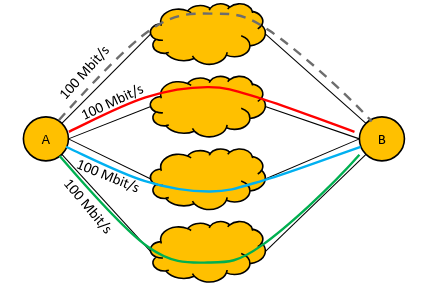
\includegraphics[width=0.4\textwidth]{pictures/3/rsvp_protection.png}
	\caption{Esempio di protezione con RSVP-TE}
\end{figure}
È possibile anche creare LSP di backup per proteggere il traffico in caso di guasti, e configurare i router in modo da effettuare un failover rapido.
Ovviamente, è possibile creare schemi di backup 1:1 o 1:N, a seconda delle esigenze di protezione e dei costi associati.
Con questi sistemi è possibile creare sistemi di recupero dai fallimenti con tempi inferiori di diversi ordini di grandezza rispetto a quelli ottenibili con il routing IP.
\section{Virtual private networks (VPN)}
Le vpn sono una estensione geografica di reti private, costruite come overlay su una rete pubblica, tipicamente internet o reti MPLS di ISP.
Lo spazio di indirizzamente è quindi condiviso tra i vari siti.
Ci sono tre categorie principali di vpn:
\begin{itemize}
	\item \textbf{Trusted VPN}:tipicamente gestite da un ISP (anche per aspetti di sicurezza). I cammini di rete possono essere forzati (quality of service). Non c'è cifratura.
	Può essere sovrapposta a una rete MPLS o a una rete IP.
	\item \textbf{Secure VPN}: tipicamente gestite da specifici provider di VPN, o configurata direttamente dai sistemisti dell'azienda.
	I cammini di rete non possono essere forzati, ma c'è cifratura.
	\item \textbf{Hybrid VPN}: combina caratteristiche di trusted e secure VPN, tipicamente gestita da ISP.
\end{itemize}
\subsection{MPLS Virtual Private LAN Service}
Una soluzione per creare VPN di layer 2 è il \textbf{MPLS Virtual Private LAN Service (VPLS)}.
Tipicamente utilizzato per connettere datacenter. Al livello logico opera come una serie di switch interconnessi (ovvero i PE)
\begin{figure}[H]
	\centering
	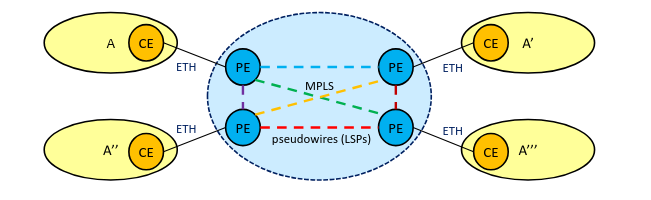
\includegraphics[width=0.9\textwidth]{pictures/3/vpls.png}
	\caption{Esempio di MPLS Virtual Private LAN Service (VPLS)}
\end{figure}\noindent
I frame ethernet vengono direttamente trasportati in pacchetti MPLS, senza incapsulamento IP.
I CE (customer edge) comunicano con i PE (provider edge) tramite frame ethernet.
I PE dunque inoltrano questi frame tramite interfacce virtuali, a cui vengono associati degli pseudocavi (tramite LSP) come se fossero link al livello 2.
I PE quindi si comportano esattamente come fossero switch al livello 2. Il meccanismo di forwarding funziona come le reti a livello 2, unicast in caso di 
destinazioni con indirizzi noti o broadcast in caso di destinazioni sconosciute.
\subsection{IP tunneling}
Permette di creare VPN di layer 3, incapsulando i pacchetti IP in pacchetti IP in un meccanismo di tunneling.
Il trasporto dei pacchetti IP avviene in maniera trasparente usando l'incapsulamento e cifratura se necessario.
Utile per creare reti IP private usando una rete IP pubblica, come ad esempio internet.
\begin{figure}[H]
	\centering
	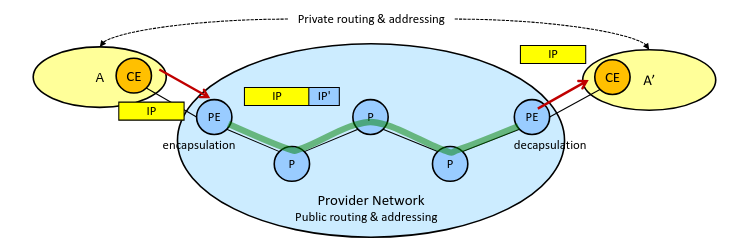
\includegraphics[width=0.9\textwidth]{pictures/3/ip_tunneling.png}
	\caption{Esempio di IP tunneling}
\end{figure}\noindent
Il PE encapsula i pacchetti IP che arrivano dalla rete private (incluso l'header IP originale) come payload di un nuovo pacchetto IP, con un nuovo header IP che viene mandato sulla rete pubblica.
L'indirizzo di destinazione del pacchetto originale sarà un indirizzo privato non raggiungibile sulla rete pubblica, ma l'indirizzo di destinazione del nuovo pacchetto sarà un indirizzo pubblico raggiungibile sulla rete pubblica (del PE target).
Il tunneling risulta meno efficiente e flessibile rispetto a VPLS, ma può essere usato su una rete IP standard, senza richiedere sostanziali modifiche ai dispositivi di rete.
Inoltre, permette di utilizzare reti gestite da provider diversi, il che invece è molto complicato con VPLS.
\section{Virtual Local Area Networks (VLAN)}
\begin{figure}[H]
	\centering
	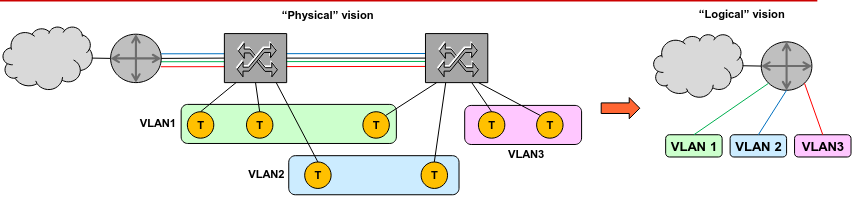
\includegraphics[width=0.9\textwidth]{pictures/3/vlan.png}
	\caption{Esempio di Virtual Local Area Networks (VLAN)}
\end{figure}\noindent
Create per avere maggiore flessibilità nella gestione di reti LAN in grossi ambienti, come ad esempio campus o edifici aziendali.
Nell'esempio in figura mostriamo una rete LAN fisica divisa in tre VLAN sullo stesso link fisico.
\begin{figure}[H]
	\centering
	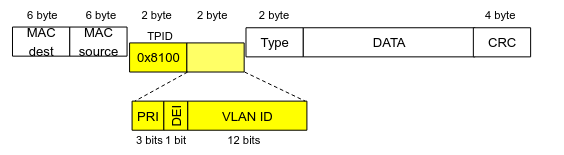
\includegraphics[width=0.9\textwidth]{pictures/3/ethernet_vlan.png}
	\caption{Esempio di incapsulamento di frame ethernet in una VLAN}
\end{figure}\noindent
Il traffico sulle varie VLAN viene distinto attraverso 4 byte aggiuntivi nella trama ethernet, detti VLAN tag, che contengono:
\begin{itemize}
	\item \textbf{VLAN identifier} (12 bit): identifica la VLAN a cui appartiene il frame.
	\item \textbf{Priority bit} (3 bit): usato per la QoS, permette di classificare i frame in base alla priorità (standard 802.1p).
	\item \textbf{Discard eligibility bit} (1 bit): usato per la QoS, indica se il frame può essere scartato in caso di congestione.
\end{itemize}
Le interfacce degli switch devono essere a conoscenza delle VLAN, in modo da poter distinguere i frame e instradarli correttamente.
Le interfacce dei terminali, invece, possono essere a conoscenza o meno delle VLAN, a seconda delle esigenze di configurazione.
Nel caso ne siano a conoscenza, il vlan tag viene aggiunto dalla porta dello switch a cui è connesso il terminale.
L'utilizzo di VLAN porta quindi ad avere facile riconfigurazione della rete, dato che è possibile spostare un terminale da una VLAN all'altra semplicemente cambiando la configurazione dello switch.
Inoltre, permette di avere una maggiore sicurezza, dato che è possibile isolare il traffico tra le VLAN.
